\section{Les projets}

J'ai donc, comme expliqué précédemment, travaillé sur quatre projets au moment de l'écriture de ce rapport.
Le premier est la SIB\footnote{Société Ivoirienne de Banque}, Palatine, Banque Dupuy de Parseval et ABE\footnote{Agricultural Bank of Egypt}.

\subsection{SIB}

La Société Ivoirienne de Banque est une des filiales de groupe bancaire marocain Attijariwafa Bank. C'est l'une des banques les plus importantes en côte d'ivoire.\\

La mission était d'ajouter une nouvelle note système qui permettrait d'évaluer le risque crédit sous forme de notation en se basant sur une note système existante et en rajoutant un questionnaire.\\

Il fallait donc dans un premier temps créer un EDW. Un EDW est un document de type Word propre à Anadefi qui permet de relier les réponses des utilisateurs à la grille de notation correspondante.

\begin{figure}[h]
\centering
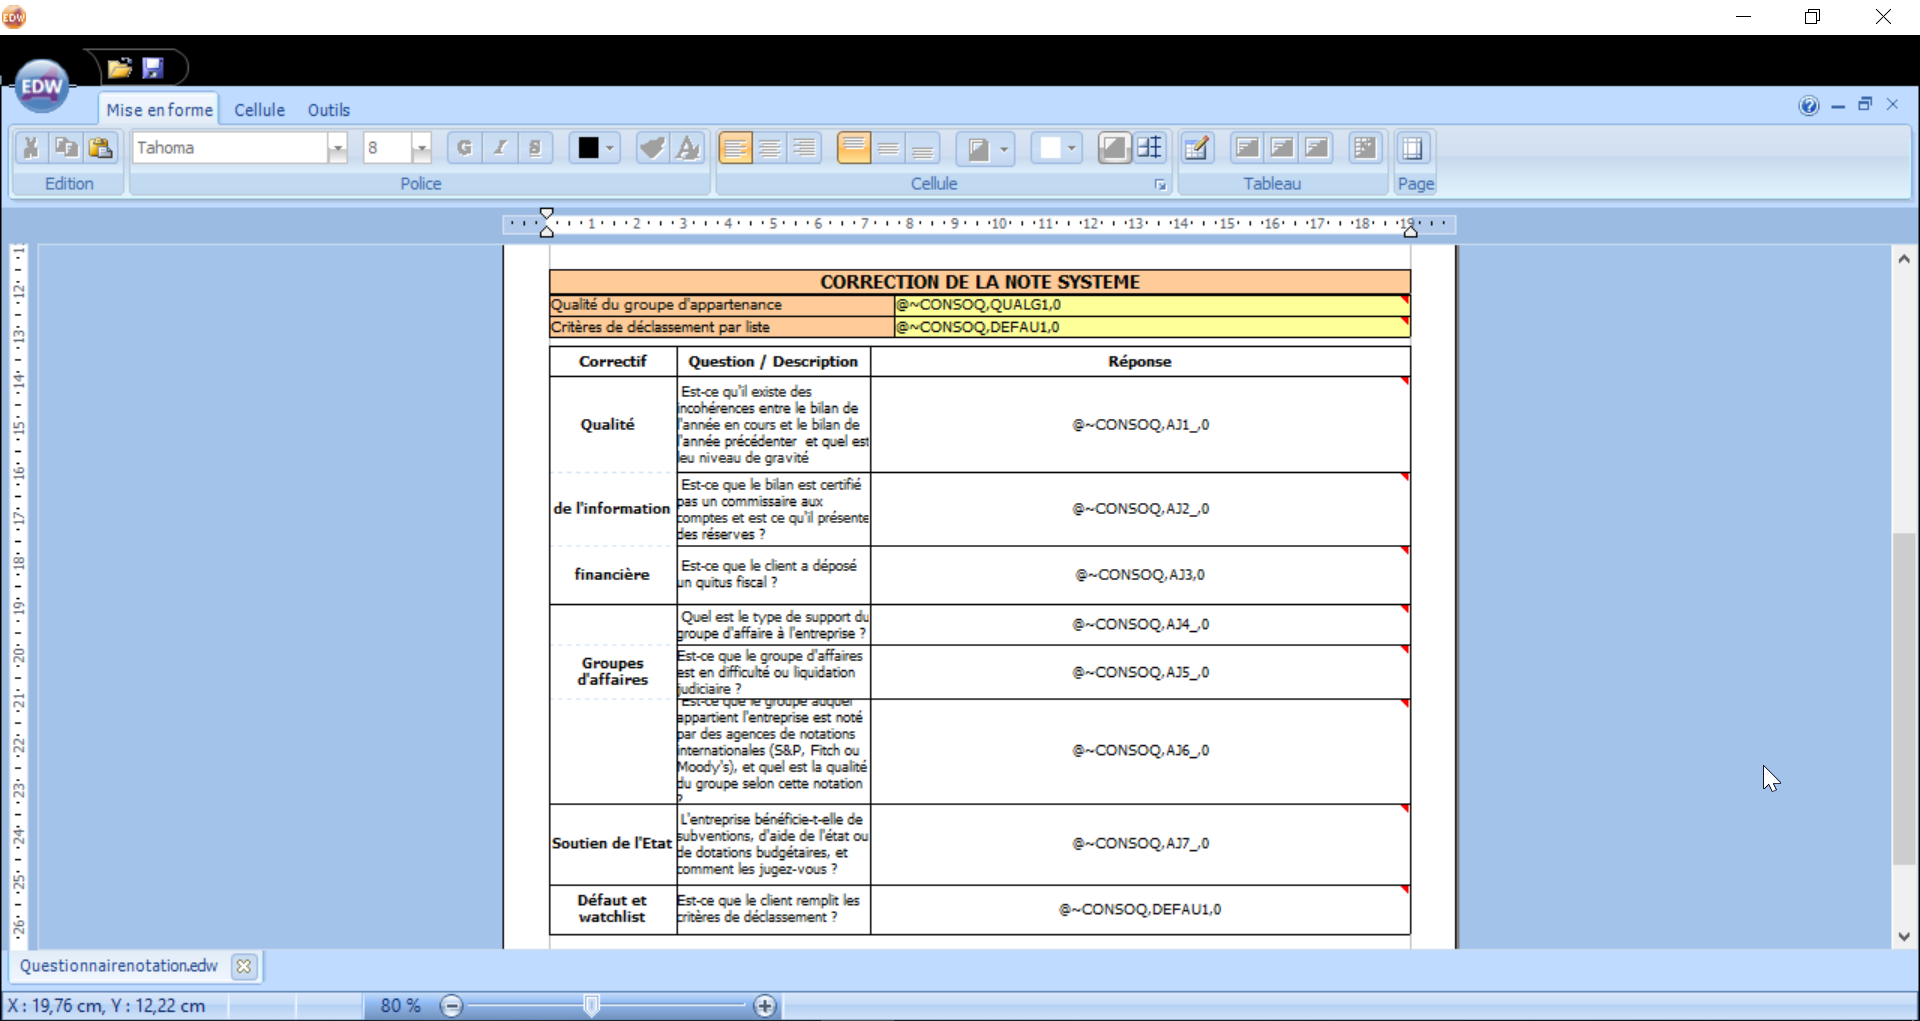
\includegraphics[scale=0.5]{resources/edw.png}
\caption{EDW questionnaire}
\label{edwSIB}
\end{figure}

Les réponses aux questions seront donc reprises grâce aux codes que vous pouvez voir dans la colonne "Réponse" et c'est dans l'outil Admin2000.exe qu'on va les traiter.\\

Dans l'outil Admin2000.exe on sélectionne la grille de cotation en question. Pour relier les questions et réponses aux EDW on utilise le code de la grille puis le code de la cellule.
Chaque réponse à une valeur différente, cette valeur a été exprimée par le client dans le cahier des charges. Pour attribuer la valeur à la réponse sélectionnée il faut faire des fonctions booléennes comme dans l'exemple suivant : 


\begin{figure}[ht]
\centering
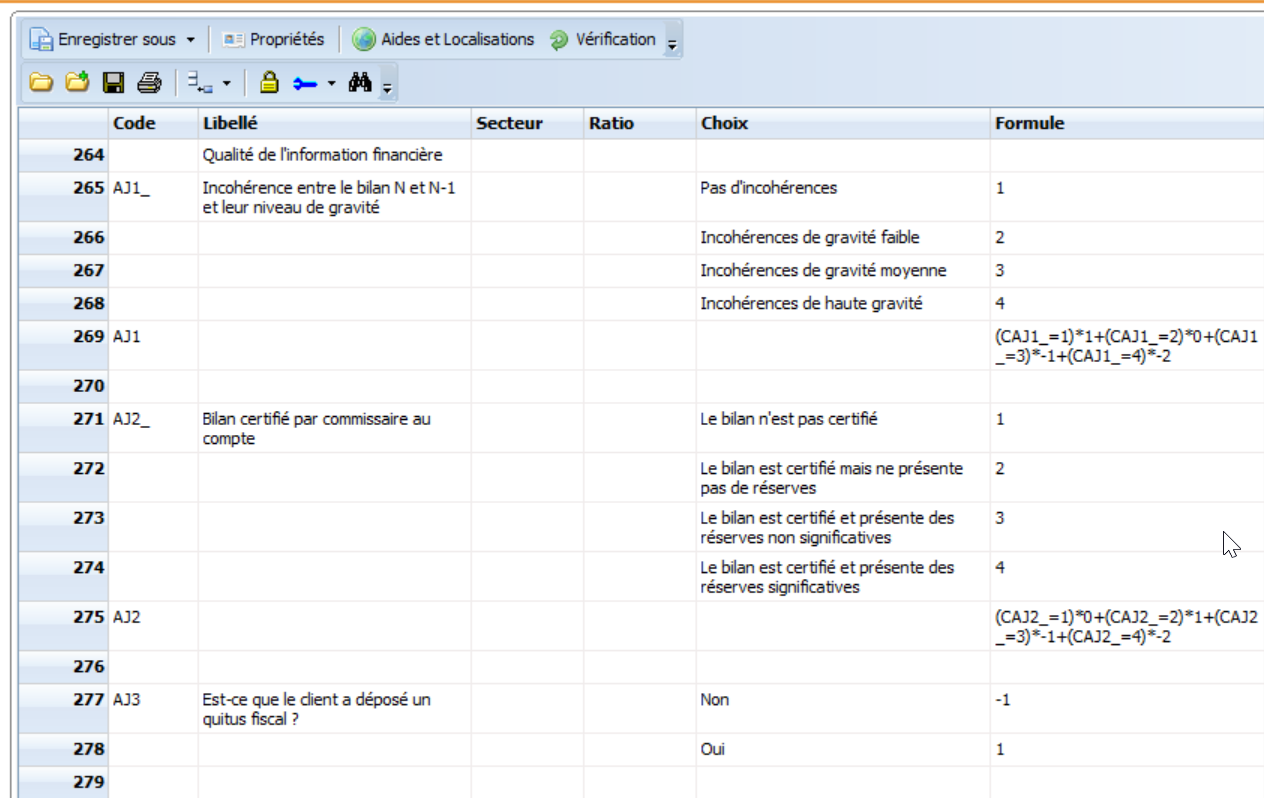
\includegraphics[scale=0.5]{resources/fctBoolAdmin.png}
\caption{Fonction booléen}
\label{fctBool}
\end{figure}


On trouve donc les réponses à une question posée. Chaque question est dans un ordre précis accompagnée d'un numéro. Le numéro de question est multiplié par la valeur de la question (qui nous a été donnée par le client) si et seulement si elle est cochée dont l'intérêt d'utiliser les fonctions booléens.\\

Une fois que toutes les questions sont reliées, on va additionner le tout pour obtenir un résultat numérique et c'est ce résultat qui va constituer une partie de la note. Cela se fera dans la grille de notation.

\begin{figure}[ht]
\centering
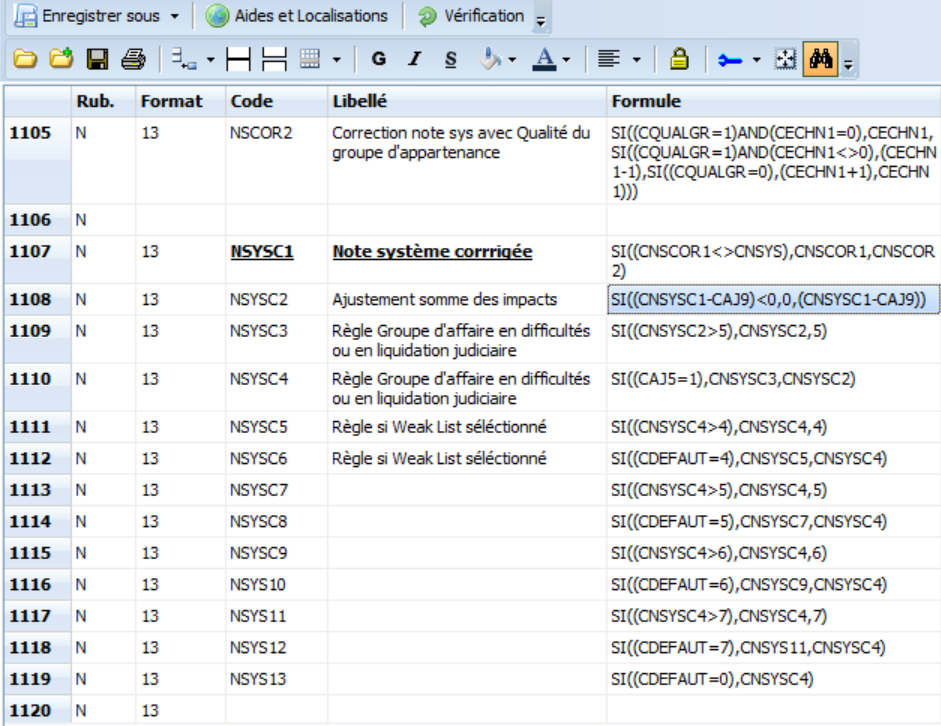
\includegraphics[scale=0.6]{resources/grille_notation.png}
\caption{Grille de notation}
\label{grCot}
\end{figure}

Dans cette grille, nous allons mettre en place toutes les conditions exprimées par le client qui feront qu'en fonction de la réponse de chaque question on obtienne une note. Par exemple si la note obtenue en remplissant le questionnaire vaut 3 mais qu'on a répondu "non" à la question 4 alors on prendra la pire note entre la note système actuelle et la note F\footnote{Une notation exprimée par le client}. Il y a pleins d'autres conditions de la sorte mais je ne vais pas détailler d'avantages, si besoin, se référer à l'annexe 1.\\

Une fois terminée, il a fallu tester une vingtaine de cas et en cas d'anomalie il fallait naturellement corriger puis retester. Une étape assez longue et difficile car c'est un travail qui demande beaucoup de rigueur et de patiente.\\

Après avoir testé, grâce à l'outil packager.exe je récupère le nouveau paramétrage l'envoi au responsable projet qui va valider et livrer la recette.\\

Sur ce projet, il n'y avait pas de problème en particulier, mais le temps de comprendre à quoi correspond chaque interface, comment écrire le plus clairement et le plus proprement possible les règles de gestion, ce n'était pas si simple surtout quand c'est la première fois qu'on fait ce genre d'exercice.


\subsection{Palatine}

Palatine est l'une des plus anciennes banques françaises encore en activité. Elle est de taille intermédiaire et elle est au service des entreprises de taille intermédiaires et de la gestion de patrimoine. Elle fait partie du groupe BPCE.\\

La banque de Palatine a contacté Sopra Banking Software pour une prestation d'extraction de données depuis leur base de données Anadefi car ils souhaitaient migrer leurs données vers un nouvel outil qui a été développé en interne par le groupe.\\

Ce qui était prévu initialement, c'était de créer trois fichiers en .ini à partir de l'outil "DefExport.exe", qui allaient ensuite être insérés dans l'outil "MoteurDexport.exe". Cet outil va par la suite, générer les trois fichiers en .csv contenant toutes les données financières demandées par Palatine.\\

La première étape est donc de monter un environnement Anadefi similaire à celui de Palatine, ce qui comprend la même version du logiciel, la même base de données, avec le même paramétrage entre autre.\\

La deuxième étape était de créer les fichiers .ini à l'aide de l'outil "DefExport.exe" dans lesquels on va indiquer les grilles financières que l'on souhaite extraire, la date des exercices, les données financières à partir des codes fournis et toute autre condition.\\

La troisième étape était donc de tester si les fichiers en .ini crées sont correctes et s'ils exportent bien les données demandées. C'est donc à ce moment que nous nous sommes aperçu qu'il y avait un gros soucis de volumétrie et que trois fichiers en .ini ne suffisaient pas pour exporter la totalité des données demandées.\\

Nous avons donc décidé d'appliquer plusieurs filtres qui permettaient de repartir les données sur plusieurs fichiers. Le premier filtre était le découpage par grilles, il y avait cinq grilles différentes. Par la suite nous avons appliqué le découpage par bureau en fonction du nombre de dossiers. Certains bureaux étaient composés d'environ 2000 dossiers et d'autres à peine une centaine, il a donc fallu donc essayer de repartir au mieux les bureaux sur les fichiers pour trouver un bon équilibre, sans qu'un fichier soit beaucoup trop volumineux par rapport à un autre. Prendre uniquement les cinq derniers exercices et prendre uniquement les exercices dont le numPartenaire\footnote{un numéro d'identifiant unique} est renseigné. En découpant par tous ces filtres nous sommes passés de trois à vingt.\\

Comme mentionné plus haut, c'est avec l'outil "DefExport.exe" qui permet de créer les fichiers d'extraction en .ini.
Dans cet outil on va définir le nom du fichier, le séparateur qui sera utilisé dans le .csv, la sélection d'une ou plusieurs grilles, la date d'échéance des exercices, le nom du fichier .csv généré et son contenu, les différents filtres qui sont demandés par le client et toute information qui serait dans le fichier .ini et dans le .csv. Au moment de la sélection des codes, il faut créer un champs dans lequel on va indiquer le nom du champs, le type de la donnée et la valeur de la donnée.

\begin{figure}[ht]
\centering
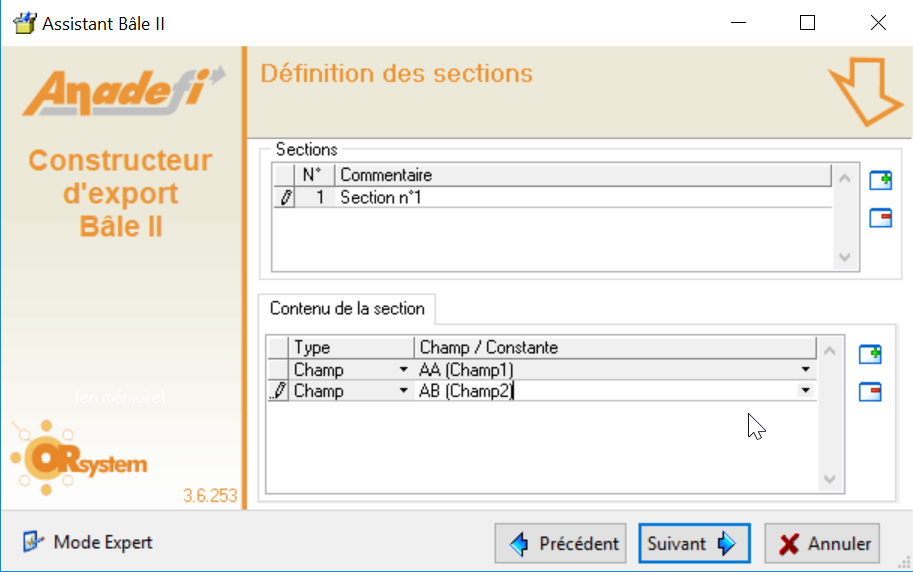
\includegraphics[scale=0.6]{resources/champ1.png}
\caption{Création des champs}
\label{champ1}
\end{figure}

\begin{figure}[ht]
\centering
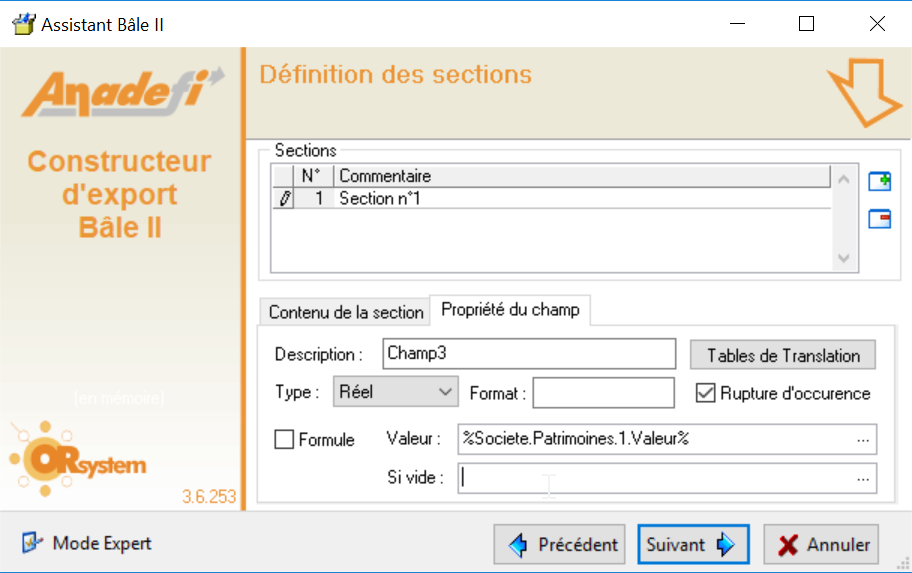
\includegraphics[scale=0.6]{resources/champ2.png}
\caption{Renseignements des champs}
\label{champ2}
\end{figure}

Le problème était qu'il fallait répéter cette action pour chaque champ c'est-à-dire 321 multipliées par 20 ce qui est très très long et le risque d'erreur est très élevé.\\

J'ai donc décidé de faire un script en Python. Pour créer un fichier j'aurai pu prendre n'importe quel autre langage mais j'ai choisis le Python pour sa simplicité syntaxiquement parlant mais aussi, le fait que je n'ai pas pratiquer du Python durant cette année contrairement au langage Java.\\

J'ai tout d'abord fait une requête SQL pour pouvoir afficher, copier et coller tous les codes qui allaient être utilisés. Par la suite, j'ai utilisé une expression régulière pour que les codes puissent être entre guillemet comme dans la figure suivante :


\begin{figure}[ht]
\centering
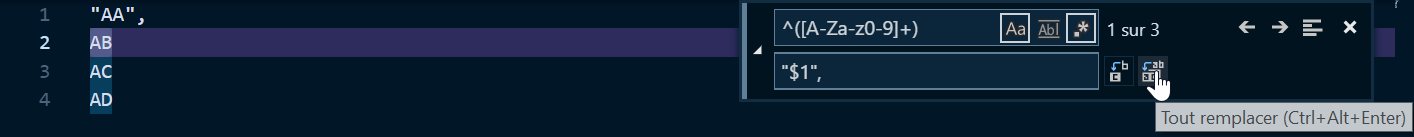
\includegraphics[scale=0.6]{resources/regex.png}
\caption{Expression régulière}
\label{regex}
\end{figure}

J'ai donc créé une liste contenant les codes en rajoutant des crochets. J'ai ensuite effectué le même procédé avec les différents bureaux. Arrivé à ce moment, j'avais tous les éléments pour faire mon script. J'ai donc eu à faire deux boucles imbriquées, une condition et une fonction qui me permet de créer des fichiers pour faire mon script. Pour tester les fichiers .ini créent à partir de mon script, j'ai dû les tester directement dans l'outil qui permet de faire l'extraction "Moteurexport.exe" si le fichier .ini ne généré pas d'erreur ni d'avertissement et qui me donnait en sortie mon fichier .csv avec des données alors le script était bon. Pour tester, je n’avais plus vingt fichiers .ini mais seulement quelques lignes de codes que j'ajustais au fur et mesure des erreurs trouvées dans les fichiers générés. Au final j'ai gagné beaucoup de temps et puis même à l'avenir pour un autre projet d'extraction mes scripts sont réutilisables et facilement ajustable.

Une fois terminée, j'ai écrit une documentation indiquant les noms des fichiers .csv qui seront générés, en fonction de leur contenance : les grilles, bureaux, le type de bilan, le nombre de dossiers à extraire pour chaque fiche et pour finir l'intitulé des codes pour qu'ils puissent savoir à quoi correspond une valeur présente dans le .csv.

\subsection{ABE}

Agricultural Bank of Egypt est une banque de la filiale National Bank of Egypt qui a été fondé en 1902.
Elle est spécialisée pour les particuliers initialement issus de l'agriculture mais s'est diversifié au fur et mesure des années.\\

Nous avions reçu une offre commerciale pour une modification et correction d'un paramétrage existant.
Le responsable de projet a rédigé la proposition commerciale. J'avais pour mission d'écrire les spécifications à partir du cahier des charges.\\

Ce cahier des charges était entièrement en anglais, il n'y a aucun interlocuteur qui parle français chez ABE. Cela n'a pas été un problème car j'ai une certaine aisance en anglais. À l'aide de mon responsable j'ai donc écrit en français chaque besoin exprimé par le client. Je l'ai rédigé en français car c'est un document qui restera en interne au sein du Pôle Service d'Anadefi. Vous trouverez en annexe une partie de la spécification. À ce jour, on attend que l'ABE signe la proposition commerciale pour pouvoir démarrer les travaux.



\subsection{Banque Dupuy de Parseval}

Banque Dupuy de Parseval est une banque, tout comme Palatine du groupe BPCE. Elle est présente dans la région du Languedoc - Roussillon et est au service principalement des entreprises de la région.\\

Pour les mêmes raisons que la banque de Palatine, elle souhaite extraire tous ces données de la base Anadefi pour les importer dans l'outil développé par le groupe BPCE.\\

Pour ce projet, j'ai écrit une grosse partie de la proposition commerciale car ayant travaillé sur Palatine juste avant, je connaissais les différentes étapes, prérequis, la prestation en elle même et les éléments à livrer. Dans cette proposition, j'ai écrit les différentes étapes de la prestation demandée.
La première était de définir l'objectif de la prestation. Ensuite définir les modalités qui doivent être réalisées et celle qui ne le seront pas. Les prérequis de cette extraction, dans ce cas étaient que BDP fasse une sauvegarde et un recalcule de leur base de données Anadefi. Un résumé des différentes tâches sous formes de tableau indiquant qu'est ce que le client doit fournir ou être livré et ce qu'Anadefi doit fournir ou être livré. Concernant la partie estimation du délai de la prestation, les coûts, les clauses et tout ce qui est d'ordre de l'administratif ont donc été écrites par le responsable de projet. \\

Contrairement à Palatine nous n'avons pas eu de problème de volumétrie par conséquent, on n'a pas appliqué de filtre car on ne découpait pas les données.\\

Concernant l'écriture des fichiers .ini, j'ai donc récupéré le script que j'avais fait pour la banque de Palatine, j'ai fait quelques ajustements pour que le script génère les bons fichiers .ini et donc les bonnes données dans le .csv. La phase de test a été beaucoup plus longue à cause du temps d'extraction car contrairement à Palatine, j'avais toute la base de données sur ma machine.\\

Une fois les tests effectués j'ai envoyé les fichiers .ini au responsable de projet qui par la suite, a vérifié et testé de son côté. J'ai donc entre temps écrit une documentation indiquant le contenu des fichiers.



